%!xelatex = 'xelatex --halt-on-error %O %S'

\documentclass{thuemp}
\begin{document}

% 标题,作者
\emptitle{脉冲核磁共振及成像实验研究}
\empauthor{王驰}{陈宏}

% 奇数页页眉 % 请在这里写出第一作者以及论文题目
\fancyhead[CO]{{\footnotesize 王驰:脉冲核磁共振及成像实验研究}}


%%%%%%%%%%%%%%%%%%%%%%%%%%%%%%%%%%%%%%%%%%%%%%%%%%%%%%%%%%%%%%%%
% 关键词 摘要 首页脚注
%%%%%%%%关键词
% \Keyword{}
\twocolumn[
\begin{@twocolumnfalse}
\maketitle

% %%%%%%%%摘要
% \begin{empAbstract}
% \end{empAbstract}

% %%%%%%%%英文标题、作者、摘要、关键词
% \emptitleEn{Experiments of Modern Physics in Tsinghua University}
% \empauthorEn{Chi Wang}{Heying Wang}
% \KeywordEn{keyword1, keyword2, keyword3, keyword4, keyword5}

% \begin{empAbstractEn}
% \end{empAbstractEn}

%%%%%%%%首页角注,依次为实验时间、报告时间、学号、email
\empfirstfoot{2025-05-10}{2025-06-09}{2022012259}{chi-wang22@mails.tsinghua.edu.cn}
\end{@twocolumnfalse}
]
%%%%%%%%!首页角注可能与正文重叠,请通过调整正文中第一页的\enlargethispage{-3.3cm}位置手动校准正文底部位置:
%%%%%%%%%%%%%%%%%%%%%%%%%%%%%%%%%%%%%%%%%%%%%%%%%%%%%%%%%%%%%%%%
%  正文由此开始
\wuhao 
%  分栏开始

% \section{引言}
% \enlargethispage{-3.3cm}

\section{实验内容}

本实验使用纽迈EDUMR20-015-V-I型磁共振实验仪,此型号实验仪器包含永磁体、射频发生器、接收系统以及梯度线圈系统。其中永磁体提供$0.5 ~ \text{T}$的静磁场,并借助一恒温设备维持磁体温度在$32.0 ~ \text{C^\circ}$。

实验中,首先利用自由感应衰减(Free Induction Decay, FID)信号,使用一标准油样品(大豆油)标定仪器参数。通过调节射频脉冲宽度$t_p$,使90度脉冲的FID信号幅值最大化。接着,测量样品的拉莫尔频率$f_0$,并计算出对应的核磁共振频率$\omega_0 = 2\pi f_0$。

使用硬脉冲CPMG序列(Carr-Purcel-Meiboom-Gill sequence),测量标准植物油样以及硫酸铜$\text{CuSO}_4$溶液的横向弛豫时间$T_2$:在施加90度脉冲后施加一系列180度脉冲,记录回波信号的幅值,并由此计算$T_2$。

通过反转恢复法测量$T_1$,即在施加180度脉冲后,间隔不同的时间$\tau$再施加90度脉冲,记录FID信号的幅值随$\tau$变化的曲线。通过拟合该曲线,得到$T_1$。

最后,采用自旋回波成像序列实现样品内部结构的空间分辨成像。通过调节梯度磁场实现空间编码,并重建样品内部结构图像。

\section{实验结果与分析}

\subsection{核自旋磁矩对外磁场的响应以及拉莫尔频率的测量}

\subsubsection{核自旋共振现象}

在外加静磁场条件下,原子核自旋会与外磁场相互作用,导致能级分裂。对于氢核,其能级分裂能量为:
    
\begin{equation}
\Delta E = \mu B
\end{equation}

其中$\mu$为核磁矩,$B$为外加磁场强度。在交变磁场作用下,当电磁波频率$\nu$与能级分裂频率相等时,电子自旋会发生共振跃迁,对电磁波的吸收达到极大,满足关系式:

\begin{equation}
h \nu  = \Delta E = \mu B
\end{equation}

其中$h$为普朗克常数;发生共振时,外加交变磁场的频率$\nu$称为拉莫尔(Lamour)频率,满足:

\begin{equation}
\nu = \frac{\mu B }{h} = \frac{\gamma B}{2\pi}
\end{equation}

其中旋磁比$\gamma = \frac{\mu}{\hbar}$,描述了核自旋与外磁场的耦合强度。

\subsubsection{核自旋体系对交变磁场的响应}

对核磁共振系统,可进一步考察其整体核自旋磁矩随时间演化特性:核自旋的宏观磁化矢量$\symbf{M}$在外加静磁场$\symbf{B}_0$的作用下,会沿着磁场方向发生进动。其动力学行为可用Bloch方程描述:

\begin{equation}
\begin{aligned}
    \frac{\mathrm{d} M_x}{\mathrm{d} t} &= \gamma (\symbf{M} \times \symbf{B'})_x - \frac{M_x}{T_2} \\
    \frac{\mathrm{d} M_y}{\mathrm{d} t} &= \gamma (\symbf{M} \times \symbf{B'})_y - \frac{M_y}{T_2} \\
    \frac{\mathrm{d} M_z}{\mathrm{d} t} &= \gamma (\symbf{M} \times \symbf{B'})_z - \frac{M_z - M_z^0}{T_1}
\end{aligned}
\label{eq:bloch}
\end{equation}

其中已选取坐标轴使得外加磁场$\mathbf{B}$沿$z$轴方向,$\symbf{B'}$为外加的交变磁场,$T_1$和$T_2$分别为纵向弛豫时间和横向弛豫时间,分别对应核自旋与晶格发生能量交换,以及核自旋相互作用中,因初相位不一致而逐渐失去整体相位一致性,发生退相干。在实际实验中,由于外磁场本身不均匀性,不同位置的核自旋会感受到不同的磁场强度,导致拉莫尔频率存在空间依赖性,这使得核自旋相互作用引起的相散过程进一步加剧。横向弛豫时间可以写为$T_2^*$,满足关系:

\begin{equation}
\frac{1}{T_2^*} = \frac{1}{T_2} + \frac{1}{T_2'} = \frac{1}{T_2} + \frac{\gamma \Delta B}{2}
\end{equation}

这同时也要求,核磁共振实验中,磁场必须达到一定的均匀度才能获得较强的共振信号。

\subsubsection{匀场调节与拉莫尔频率测量}

借助于实验仪器的梯度线圈,对永磁体磁场不均匀性进行补偿;借助于实验仪器的射频线圈以及接收系统,对样品在不同频率下的功率吸收进行测量,进而确定样品的拉莫尔频率。以上实验操作均已被集成在纽迈核磁共振分析软件功能内,通过“自动主频”功能,测得拉莫尔频率

\begin{equation}
f_0 = 21.43 \text{ MHz}
\label{eq:lamor_freq}
\end{equation}

\subsection{使用CPMG序列测量横向弛豫时间$T_2$}  

\subsubsection{借助FID信号确定$90^\circ$脉冲和$180^\circ$脉冲的脉宽}    

在核磁共振实验中,$90^\circ$脉冲和$180^\circ$脉冲是两种重要的射频脉冲。$90^\circ$脉冲使得核自旋磁化矢量从平衡状态沿着$z$轴方向翻转到$x-y$平面上,形成一个横向磁化矢量;$180^\circ$脉冲则使得核自旋磁化矢量从$x-y$平面翻转到相反的方向。从Bloch方程出发进行分析,可以得到$90^\circ$脉冲和$180^\circ$脉冲的脉宽$t_p^{(90)}, t_p^{(180)}$与射频幅值$B_1$之间的关系:

\begin{equation}
t_p^{(90)} = \frac{\pi}{2\gamma B_1}, \quad t_p^{(180)} = \frac{\pi}{\gamma B_1}
\label{eq:pulse_width}
\end{equation}

其中,$B_1$为射频脉冲的幅值,$t_p^{(90)}, t_p^{(180)}$一般也记作$P_1, P_2$。

为测定$90^\circ$脉冲和$180^\circ$脉冲的脉宽,固定射频发射器功率,调节射频脉冲宽度$t_p$,可观察到样品在射频脉冲作用后发生弛豫,并产生FID信号。通过测量FID信号的幅值随脉冲宽度$t_p$的变化关系,可以确定$90^\circ$脉冲和$180^\circ$脉冲的脉宽。

借助实验软件系统,在\si{5.0 \micro \second} \~ \si{45.0\micro \second}范围内,以\si{1.0\micro \second}间隔调整脉冲宽度$t_p$,测量FID信号强度。经软件自动取数分析,得到$P_1, P_2$:

\begin{equation}
    P_1 = 17.0 \pm 0.5 \text{ }\mu\text{s}, \quad P_2 = 36.0 \pm 0.5 \text{ }\mu\text{s}
\end{equation}

\subsubsection{重复采样等待时间$T_W$的选择}

在核磁共振实验中,重复采样等待时间$T_W$是指在每次射频脉冲作用后,等待一段时间再进行下一次采样的时间间隔。$T_W$太短,则在下一次施加射频脉冲前,核自旋磁化矢量尚未完全恢复到平衡状态,导致测量结果不准确;$T_W$太长,则会延长实验时间,降低实验效率。

为选择适当的$T_W$,测量FID信号的幅值随$T_W$的变化:

\begin{table}[H]
    \centering
    \captionnamefont{\wuhao\bf\heiti}
    \captiontitlefont{\wuhao\bf\heiti}
    \caption{FID信号幅值随$T_W$的变化实验数据表}
    \label{tab:fid_TW}
    \liuhao
    \begin{tabular}{cc}
        \toprule
        重复采样等待时间$T_W / \text{ms}$ & FID信号幅值\\
        \midrule
         500 & 790.111 \\
        1000 & 988.551 \\
        1500 & 1065.768 \\
        2000 & 1101.401 \\
        2500 & 1117.401 \\
        3000 & 1124.308 \\
        \bottomrule
    \end{tabular}
\end{table}

由表\ref{tab:fid_TW}可知,FID信号幅值在$T_W = 2000 \text{ ms}$时已经接近最大值,之后幅值变化不大。因此,选择$T_W = 2000 \text{ ms}$作为重复采样等待时间。

\subsubsection{核自旋体系对CPMG序列的响应}

在CPMG序列中,首先施加一个$90^\circ$脉冲,经历一时间间隔$\tau$之后,施加一个$180^\circ$脉冲,将核自旋磁化矢量翻转到相反的方向,随后再以$2\tau$为时间间隔施加一系列$180^\circ$脉冲。

在最初的$90^\circ$脉冲作用下,核自旋磁化矢量从平衡状态沿着$z$轴方向翻转到$x-y$平面上,形成一个横向磁化矢量,并开始发生弛豫过程。其中,由于磁场的不均匀性,核自旋磁矩进动速度不一,其横向分量自然发生相散。随后,在$180^\circ$脉冲作用下,各个原子核的核自旋磁化矢量被翻转到相反的方向,并且在随后的演化过程中,此相散过程几乎发生了完全的逆转,直至在经历时间$\tau$后重新在$x-y$平面上又形成一个横向磁化矢量,产生出一个回波信号。这之后又经历时长为$\tau$的相散过程,直至又受到一个$180^\circ$脉冲,再次出现“相散-重聚”,进而在后续过程中形成一系列回波信号。

在这一过程中,核自旋磁化矢量的横向分量大小仍然会按照$T_2$这一特征时间发生衰减,并反映在回波信号的幅值上。具体地,第$n$个回波信号的幅值$U_n$与时间间隔$\tau$满足关系:

\begin{equation}
U_n = U_1 e^{-2(n-1)\tau/T_2}
\label{eq:echo_amplitude}
\end{equation}

由此,使用CPMG序列作用于样品后,记录回波信号的幅值$U_n$随时间间隔$\tau$的变化关系,可以拟合出横向弛豫时间$T_2$。

\subsubsection{横向弛豫时间$T_2$的实验测定}

在此前已选定$P_1, P_2, T_W$的基础上,选定$180^\circ$脉冲总个数$N_{\text{ECH}}=8000$,对标准油样品施加CPMG序列脉冲,记录回波信号的幅值$U_n$随时间间隔$\tau$的变化关系,得到信号:

\begin{figure}[H]
    \centering
    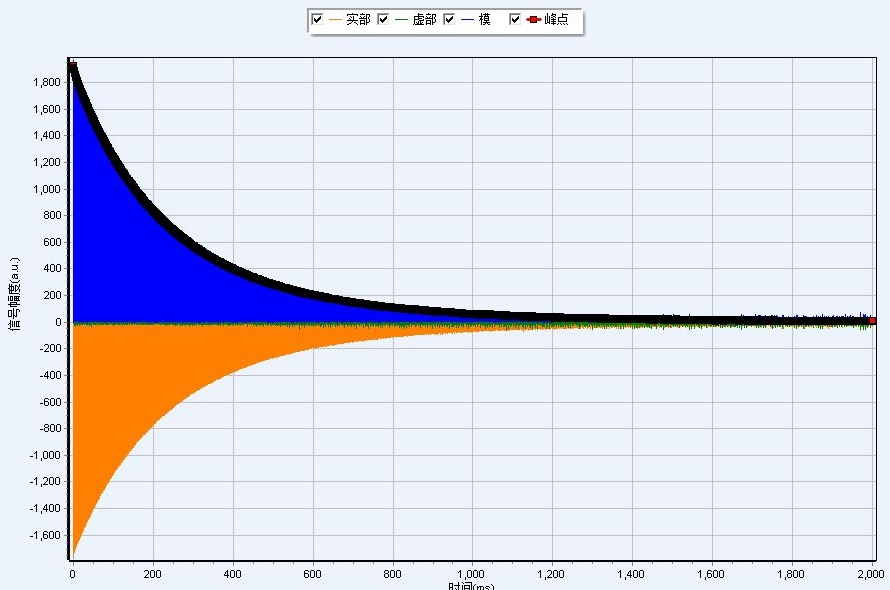
\includegraphics[width=0.8\linewidth]{../Data/pre-experiment/Oil_T2_final.JPG}
    \caption{CPMG序列下标准油样品的回波信号}
    \label{fig:cpmg_oil}
\end{figure}

使用软件进行反演,得到下图所示结果:

\begin{figure}
    \centering
    \includegraphics[width=0.8\linewidth]{../Data/pre-experiment/Oil_T2_final_analysis_plot.txt.BMP}
    \caption{CPMG序列下标准油样品的回波信号反演结果}
    \label{fig:cpmg_oil_fit}
\end{figure}

测得$T_2^{\text{Oil}} =  265.7 \text{ ms}$。

类似地,对$\text{CuSO}_4$溶液样品,使用CPMG序列进行测量。注意到由于$\text{CuSO}_4$溶液的横向弛豫时间较短,需适当减小$N_{\text{ECH}}$,以保证回波信号的幅值足够大。选取$N_{\text{ECH}}=300, T_W = 1500\text{ ms}$,记录回波信号的幅值$U_n$随时间间隔$\tau$的变化关系,得到信号:

\begin{figure}[H]
    \centering
    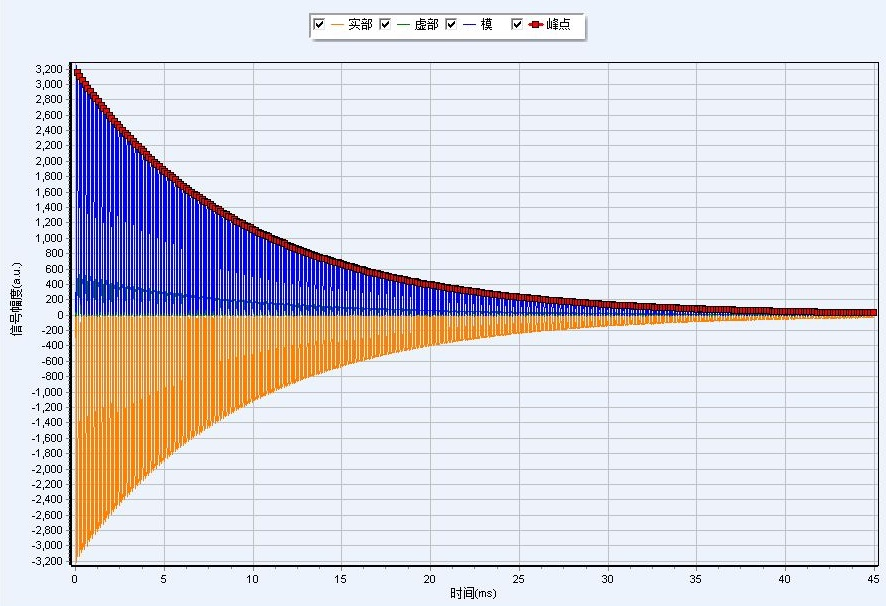
\includegraphics[width=0.8\linewidth]{../Data/pre-experiment/SLN_T2_final.JPG}
    \caption{CPMG序列下$\text{CuSO}_4$溶液的回波信号}
    \label{fig:cpmg_sln}
\end{figure}

使用软件进行反演,得到下图所示结果:

\begin{figure}[H]
    \centering
    \includegraphics[width=0.8\linewidth]{../Data/pre-experiment/SLN_T2_final_analysis_plot.txt.BMP}
    \caption{CPMG序列下$\text{CuSO}_4$溶液的回波信号反演结果}
    \label{fig:cpmg_sln_fit}
\end{figure}

测得$T_2^{\text{CuSO}_4} = 10.7 \text{ ms}$。

由此可见,在水溶液体系中,$\text{CuSO}_4$溶液的横向弛豫时间$T_2$显著小于标准油样品的$T_2$,这与理论预期一致:水中质子扩散运动加剧了横向弛豫。

\subsection{使用反转恢复(IR)序列测量纵向弛豫时间$T_1$}

\subsubsection{核自旋磁矩对IR序列的响应}

在反转恢复(IR)序列中,首先施加一个$180^\circ$脉冲,将核自旋磁化矢量翻转到相反的方向。随后,等待一段时间$t$,施加一个$90^\circ$脉冲,将核自旋磁化矢量从相反方向翻转到$x-y$平面上,形成一个横向磁化矢量,并开始发生弛豫过程,产生FID信号。此时这一信号的初始幅值$U(t)$即反映了核自旋磁化矢量在经过$180^\circ$脉冲翻转后,经历时间$t$的纵向弛豫过程所剩余的纵向磁化分量。

\subsubsection{纵向弛豫时间$T_1$的实验测定} 

在核自旋磁化矢量发生$180^\circ$翻转后的纵向弛豫过程中,核自旋磁化矢量的纵向分量大小会按照$T_1$这一特征时间发生演化,并反映在FID信号的幅值上。具体地,FID信号的幅值$U(t)$与纵向弛豫过程时间间隔$t$满足关系:

\begin{equation}
U(t) = U_0 \left(1 - 2 e^{-t/T_1}\right)
\label{eq:ir_amplitude}
\end{equation}

通过选取一系列不同的$t$值,记录FID信号的幅值$U(t)$随$t$的变化关系。由此可以拟合出纵向弛豫时间$T_1$。

对标准油样品施加IR序列脉冲,记录FID信号的幅值$U(t)$随$t$的变化关系,得到信号如下图所示:

\begin{figure}[H]
    \centering
    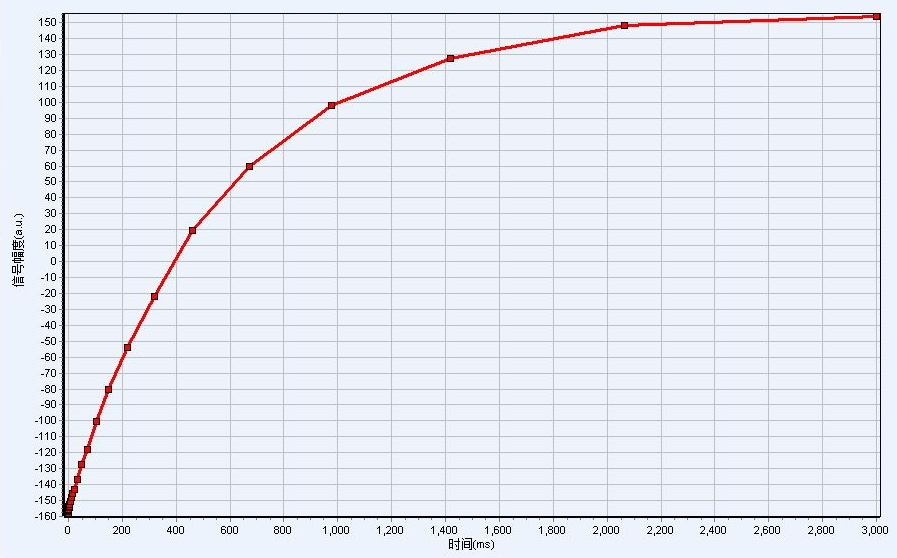
\includegraphics[width=0.8\linewidth]{../Data/pre-experiment/Oil_T1_IR_final.JPG}
    \caption{IR序列下标准油样品的FID信号}
    \label{fig:ir_oil}
\end{figure}

进行反演分析,得到下图所示结果:

\begin{figure}[H]
    \centering
    \includegraphics[width=0.8\linewidth]{../Data/pre-experiment/Oil_T1_final_analysis_plot.txt.BMP}
    \caption{IR序列下标准油样品的FID信号反演结果}
    \label{fig:ir_oil_fit}
\end{figure}

测得$T_1^{\text{Oil}} =  580 \text{ ms}$。

对$\text{CuSO}_4$溶液样品施加IR序列脉冲,记录FID信号的幅值$U(t)$随$t$的变化关系,得到信号如下图所示:

\begin{figure}[H]
    \centering
    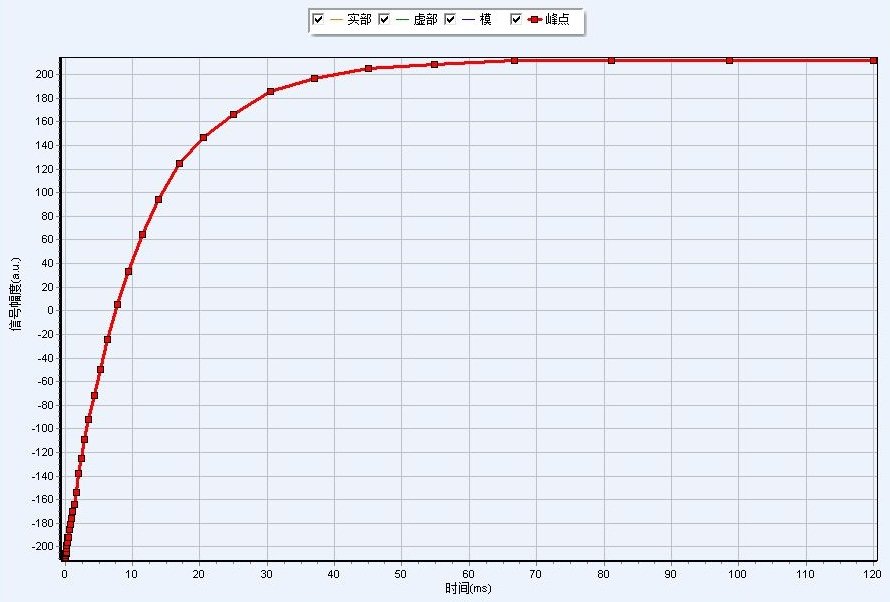
\includegraphics[width=0.8\linewidth]{../Data/pre-experiment/SLN_T1_IR_final.JPG}
    \caption{IR序列下$\text{CuSO}_4$溶液的FID信号}
    \label{fig:ir_sln}
\end{figure}

进行反演分析,得到下图所示结果:

\begin{figure}[H]
    \centering
    \includegraphics[width=0.8\linewidth]{../Data/pre-experiment/SLN_T2_final_analysis_plot.txt.BMP}
    \caption{IR序列下$\text{CuSO}_4$溶液的FID信号反演结果}
    \label{fig:ir_sln_fit}
\end{figure}

测得$T_1^{\text{CuSO}_4} =  10.7 \text{ ms}$。

可以发现,到标准油样品与$\text{CuSO}_4$溶液的纵向弛豫时间$T_1$与各自的横向弛豫时间$T_2$相比,均处在同一数量级而稍长;而$\text{CuSO}_4$溶液的纵向弛豫时间$T_1$同样远小于标准油样品的纵向弛豫时间$T_1$。


\subsection{使用自旋回波成像序列实现空间分辨成像}

\subsubsection{自旋回波序列与加权像}

在自旋回波序列中,首先施加一个$90^\circ$脉冲,经历一时间间隔$\tau$之后,施加一个$180^\circ$脉冲。在第一个$90^\circ$脉冲作用下,核自旋磁化矢量从平衡状态沿着$z$轴方向翻转到$x-y$平面上,形成一个横向磁化矢量,并开始发生弛豫过程。随后,在$180^\circ$脉冲作用下,各个原子核的核自旋磁化矢量被翻转到相反的方向,并且在随后的演化过程中,此相散过程几乎发生了完全的逆转,直至在经历时间$\tau$后重新在$x-y$平面上又形成一个横向磁化矢量,产生出一个回波信号。

在使用自旋回波序列成像时,常引入以下两个序列参数:

\begin{itemize}
    \item $T_E$:回波时间(Echo Time),即从第一个$90^\circ$脉冲到第一个回波信号的时间间隔。
    \item $T_R$:重复时间(Repetition Time),即从一个自旋回波序列开始到下一个自旋回波序列开始的时间间隔。
\end{itemize}

这其中,$T_E$即为自旋磁化矢量在$x-y$平面内发生横向弛豫的时间间隔,而$T_R$则决定自旋磁化矢量在$z$轴方向发生纵向弛豫的时间间隔。在成像中,具有不同弛豫时间$T_1,T_2$的物质对$T_E$和$T_R$变化的响应并不相同,而满足以下关系:

\begin{equation}
    S(T_E, T_R) \propto N(H) \left(1 - e^{-T_R/T_1}\right)e^{-T_E/T_2}
\end{equation}

其中$S(T_E, T_R)$为成像信号强度,$N(H)$为样品中质子密度。根据这一关系,可选取不同的$T_E$和$T_R$值,来对不同物质的成像信号进行加权:

\begin{itemize}
    \item 长$T_R$和短$T_E$:此时成像信号主要由样品中质子密度决定;
    \item 短$T_R$和短$T_E$:此时成像信号强度主要受到$e^{-T_E/T_2}$因子影响,表现为横向弛豫时间$T_2$加权像,其中高信号区域对应横向弛豫时间$T_2$较长的区域;
    \item 长$T_R$和长$T_E$:此时成像信号强度主要受到$(1-e^{-T_R/T_1})$因子影响,表现为纵向弛豫时间$T_1$加权像,其中高信号区域对应纵向弛豫时间$T_1$短的区域。
\end{itemize}

由此,可以通过调节$T_E$和$T_R$的值,来对样品内部不同物质的分布进行更细致的刻画。

\subsubsection{空间分辨成像的重建}

磁共振成像过程中,首先需要对样品施加空间编码梯度磁场,使得样品中不同位置的核自旋感受到不同的磁场强度,从而使得拉莫尔频率在空间上发生变化。通过调节梯度磁场的强度和方向,可以实现对样品内部不同位置的核自旋进行编码。结合不同梯度下获得的回波信号,可以重建出样品内部的空间分布图像。

在本实验中,先后选择了一系列不同的$T_R, T_E$取值,以一支同时装有食用油和硫酸铜溶液的试管作为样品进行成像实验,并通过纽迈核磁共振成像软件自动完成成像重建,得到如下结果:

\begin{figure}[H]
    \centering
    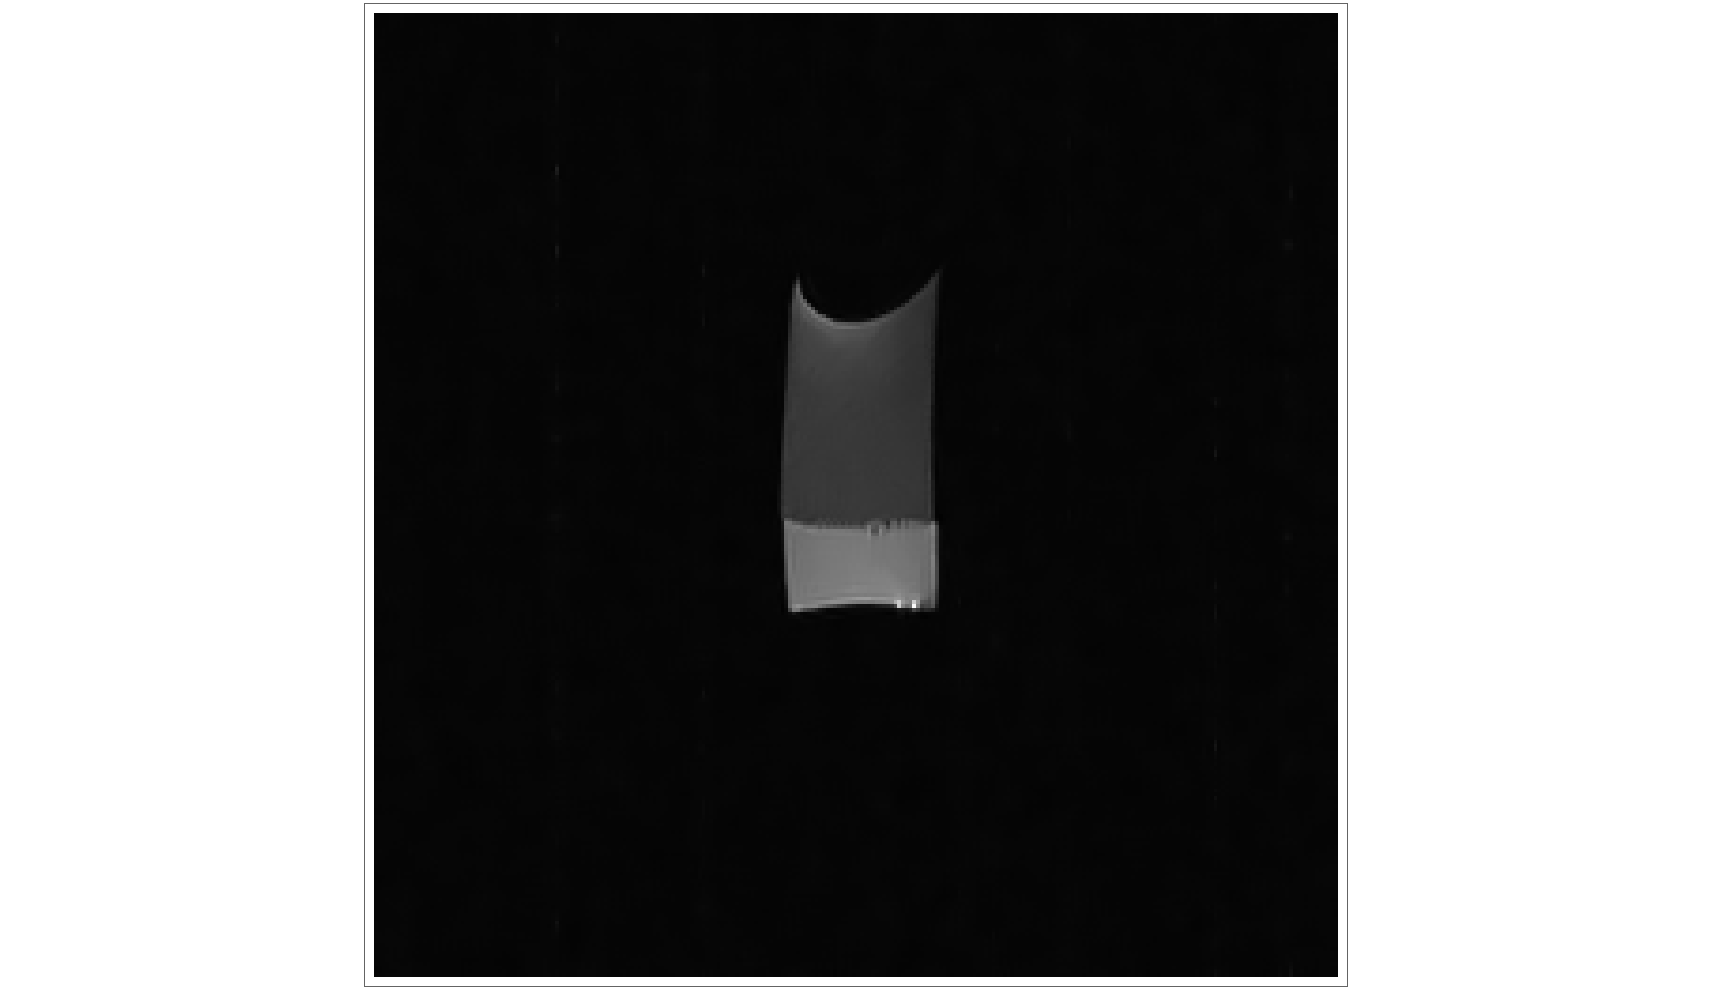
\includegraphics[width=0.8\linewidth]{../Data/pre-experiment/MRI_result_TR_0060_TE_020.bmp}
    \caption{$T_R = \text{\si{60 \micro\second}}, T_E = \text{\si{20 \micro\second}}$时的自旋回波序列共振成像结果}
    \label{fig:mri_0060_020}
\end{figure}

\begin{figure}[H]
    \centering
    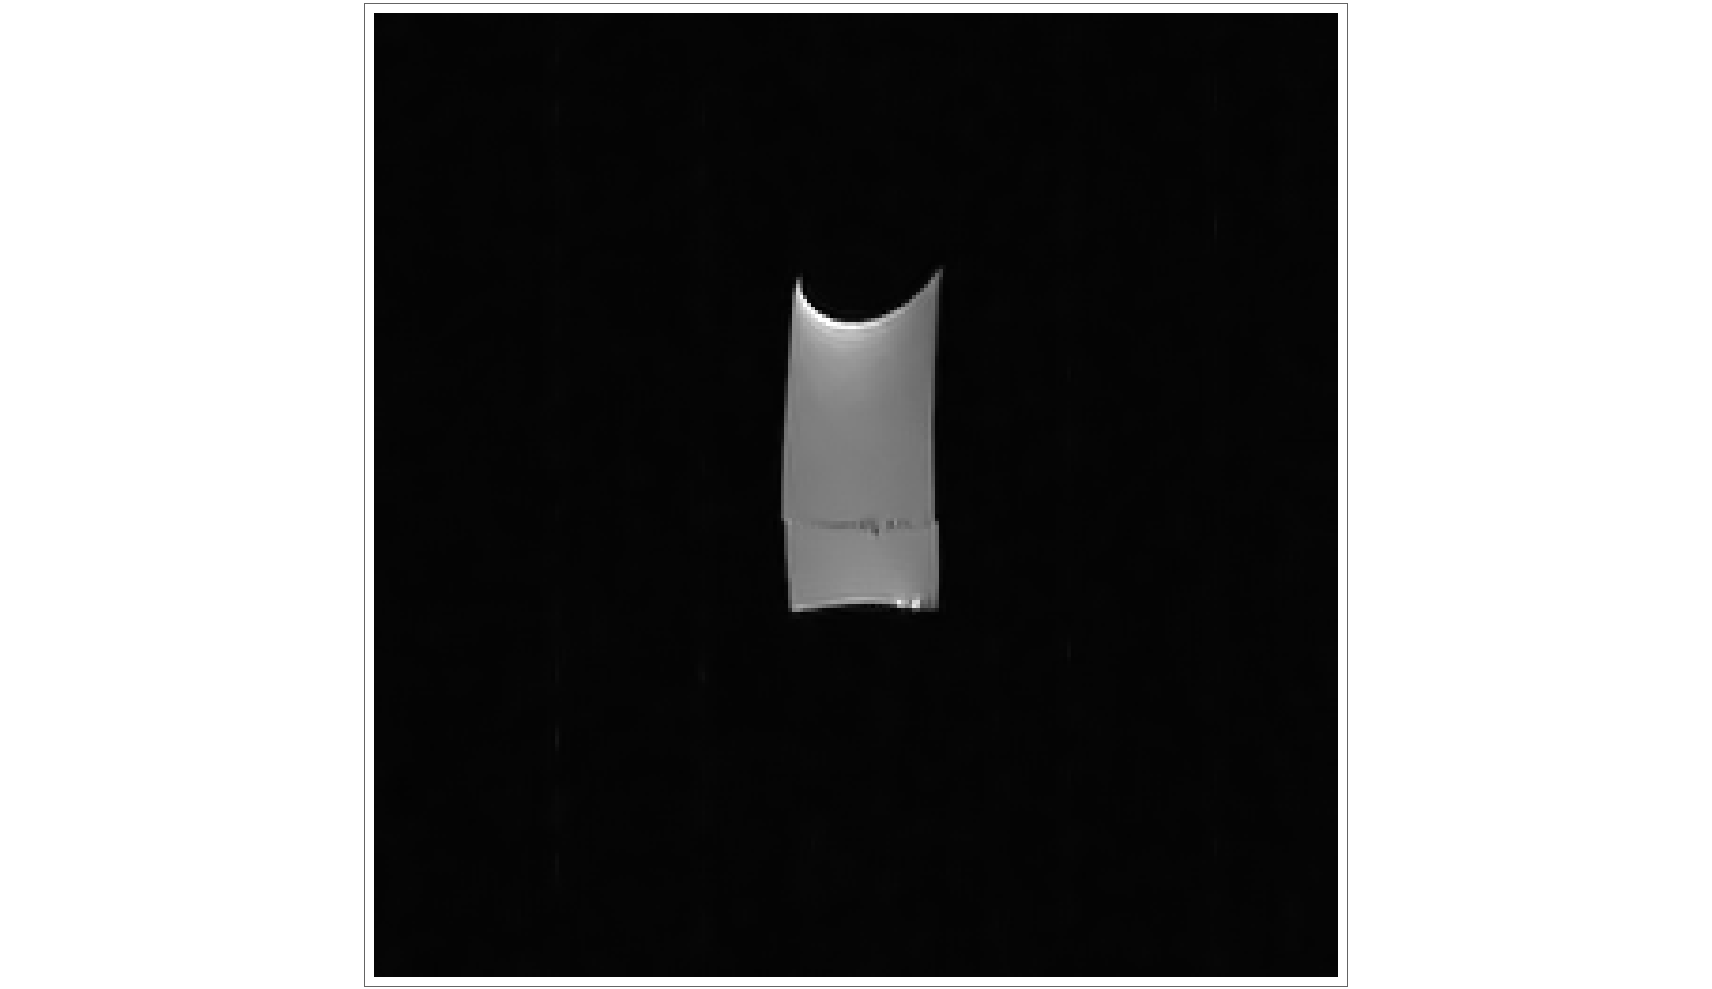
\includegraphics[width=0.8\linewidth]{../Data/pre-experiment/MRI_result_TR_0260_TE_020.bmp}
    \caption{$T_R = \text{\si{260 \micro\second}}, T_E = \text{\si{20 \micro\second}}$时的自旋回波序列共振成像结果}
    \label{fig:mri_0260_020}
\end{figure}

\begin{figure}[H]
    \centering
    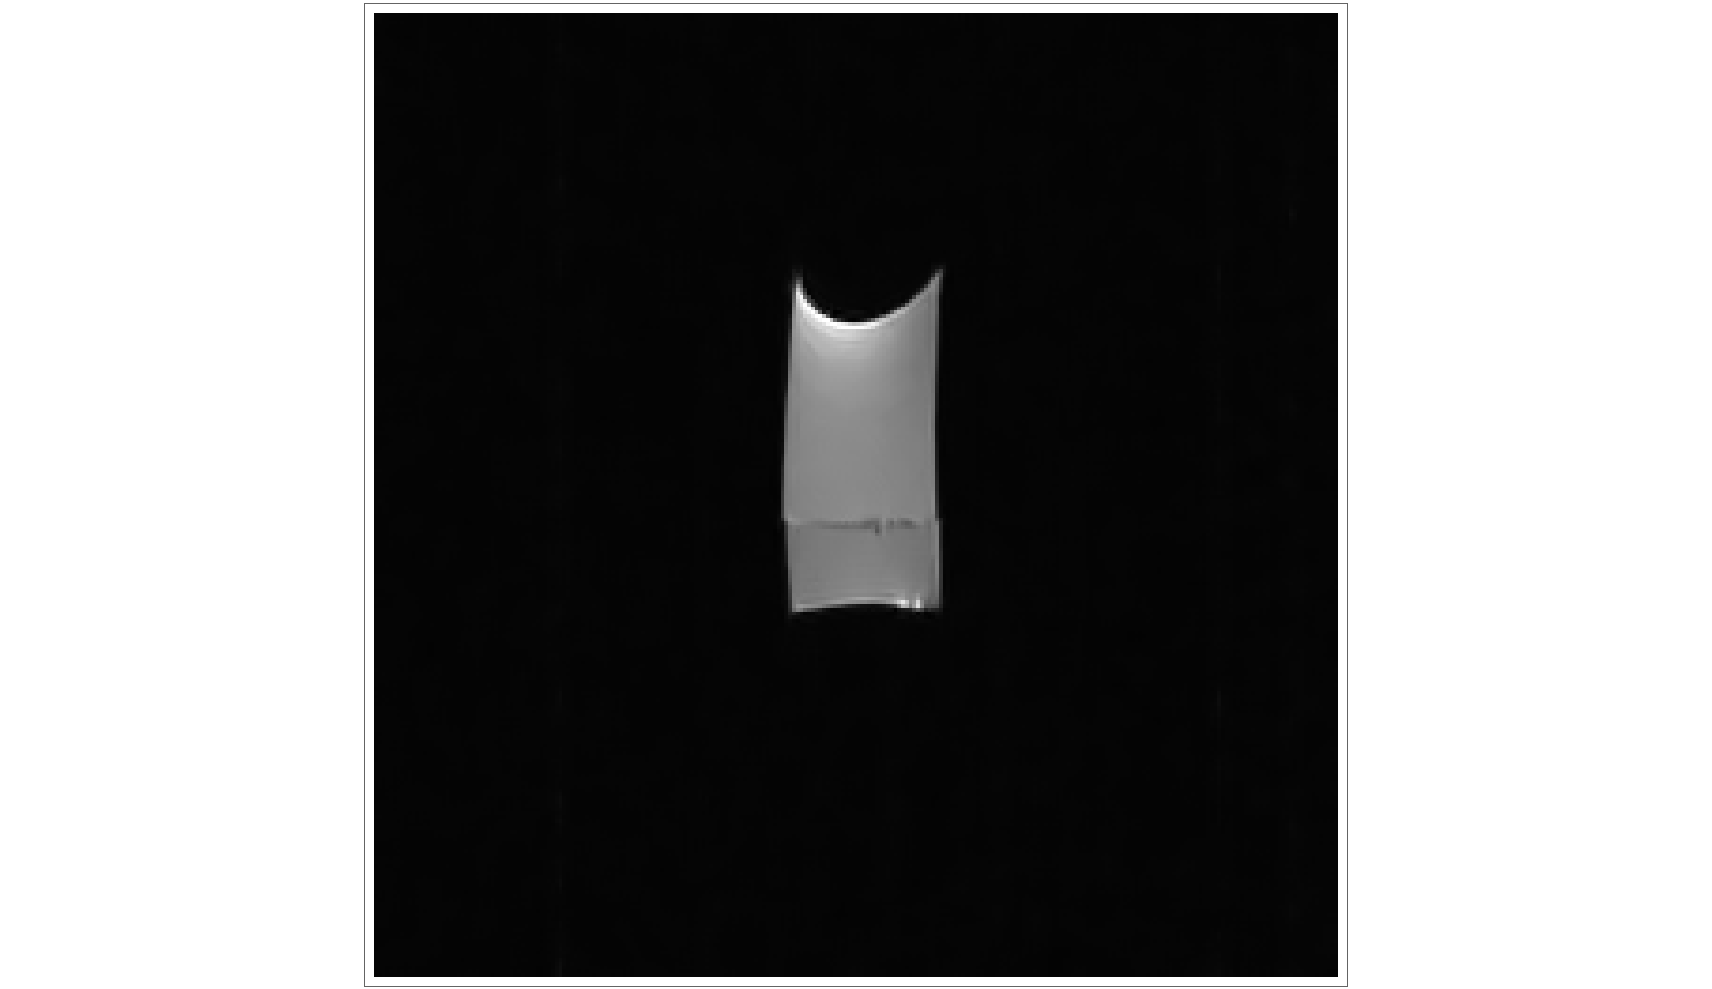
\includegraphics[width=0.8\linewidth]{../Data/pre-experiment/MRI_result_TR_0500_TE_020.bmp}
    \caption{$T_R = \text{\si{500 \micro\second}}, T_E = \text{\si{20 \micro\second}}$时的自旋回波序列共振成像结果}
    \label{fig:mri_0500_020}
\end{figure}

\begin{figure}[H]
    \centering
    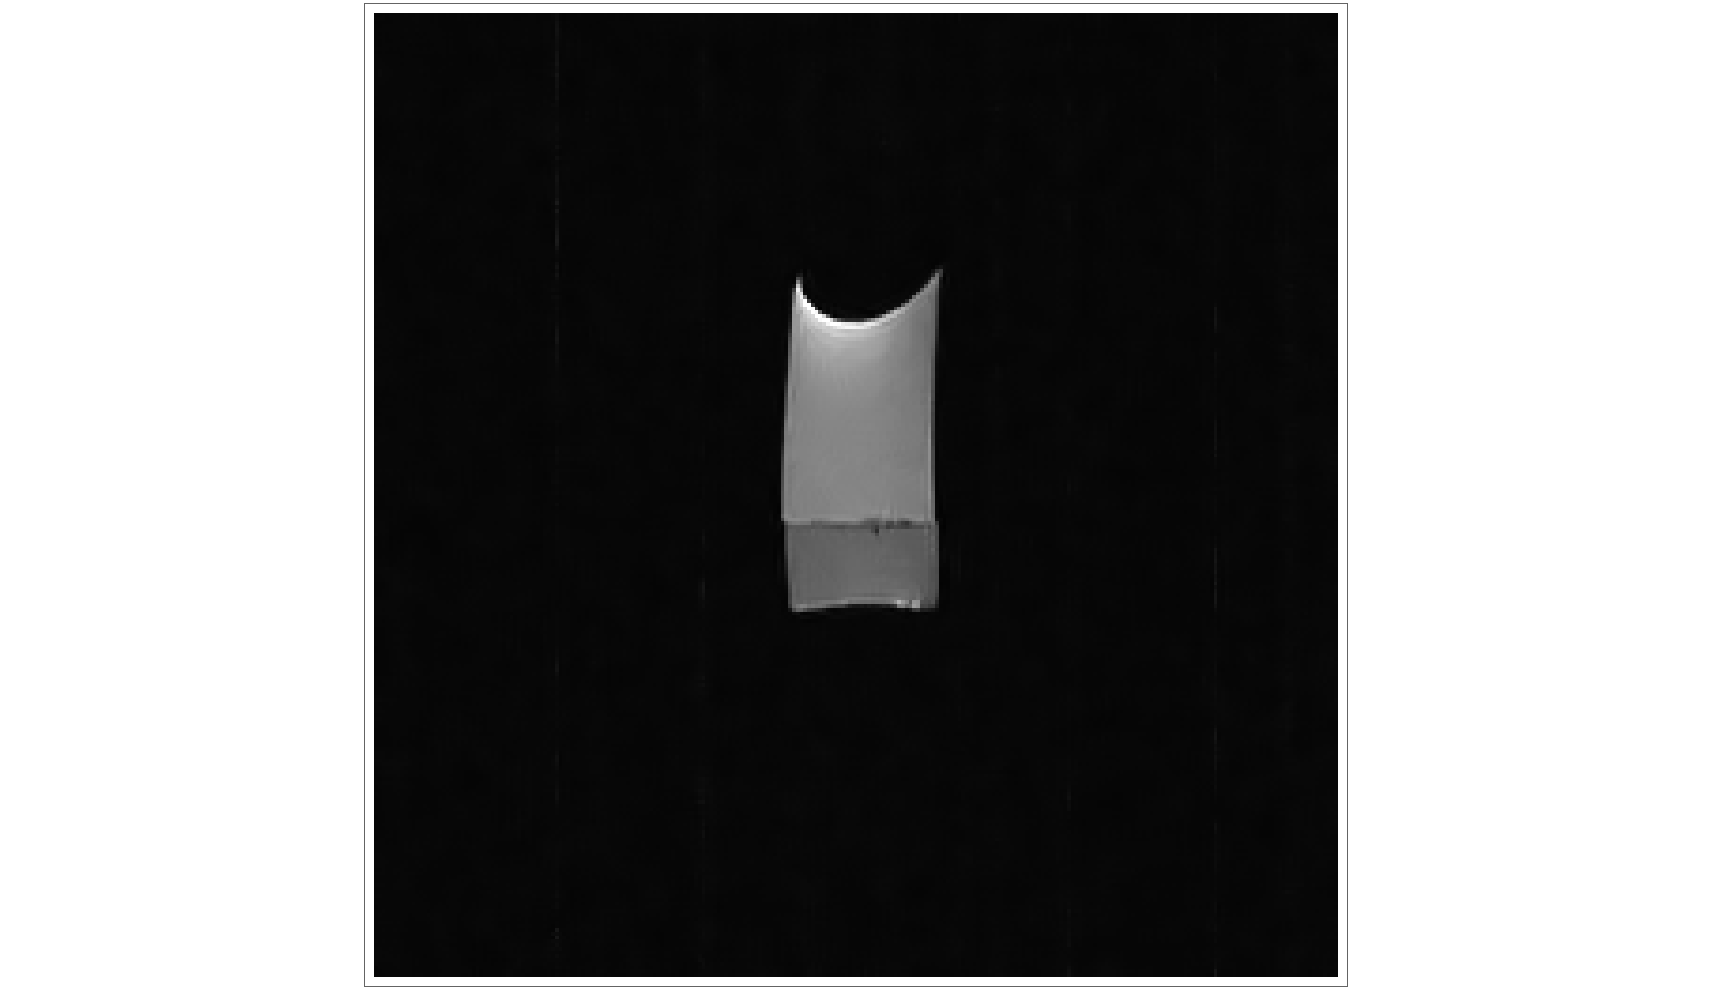
\includegraphics[width=0.8\linewidth]{../Data/pre-experiment/MRI_result_TR_0500_TE_040.bmp}
    \caption{$T_R = \text{\si{500 \micro\second}}, T_E = \text{\si{40 \micro\second}}$时的自旋回波序列共振成像结果}
    \label{fig:mri_0500_040}
\end{figure}

\begin{figure}[H]
    \centering
    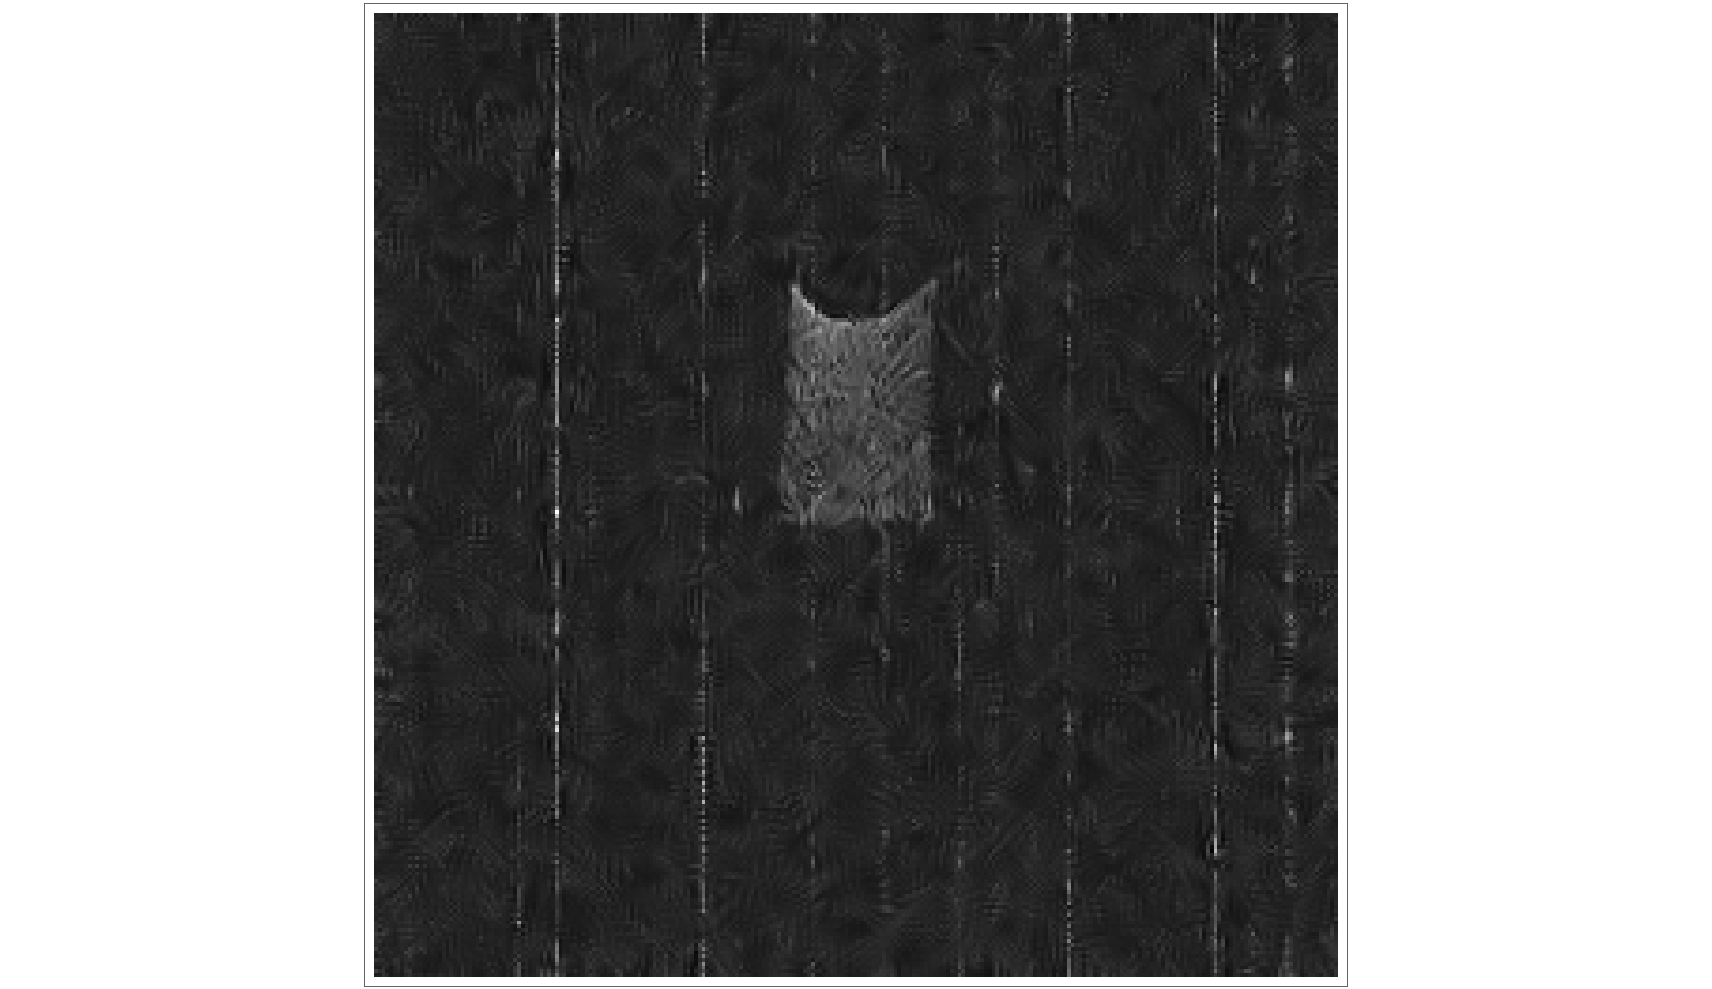
\includegraphics[width=0.8\linewidth]{../Data/pre-experiment/MRI_result_TR_0500_TE160.bmp}
    \caption{$T_R = \text{\si{500 \micro\second}}, T_E = \text{\si{160 \micro\second}}$时的自旋回波序列共振成像结果}
    \label{fig:mri_0500_160}
\end{figure}

\begin{figure}[H]
    \centering
    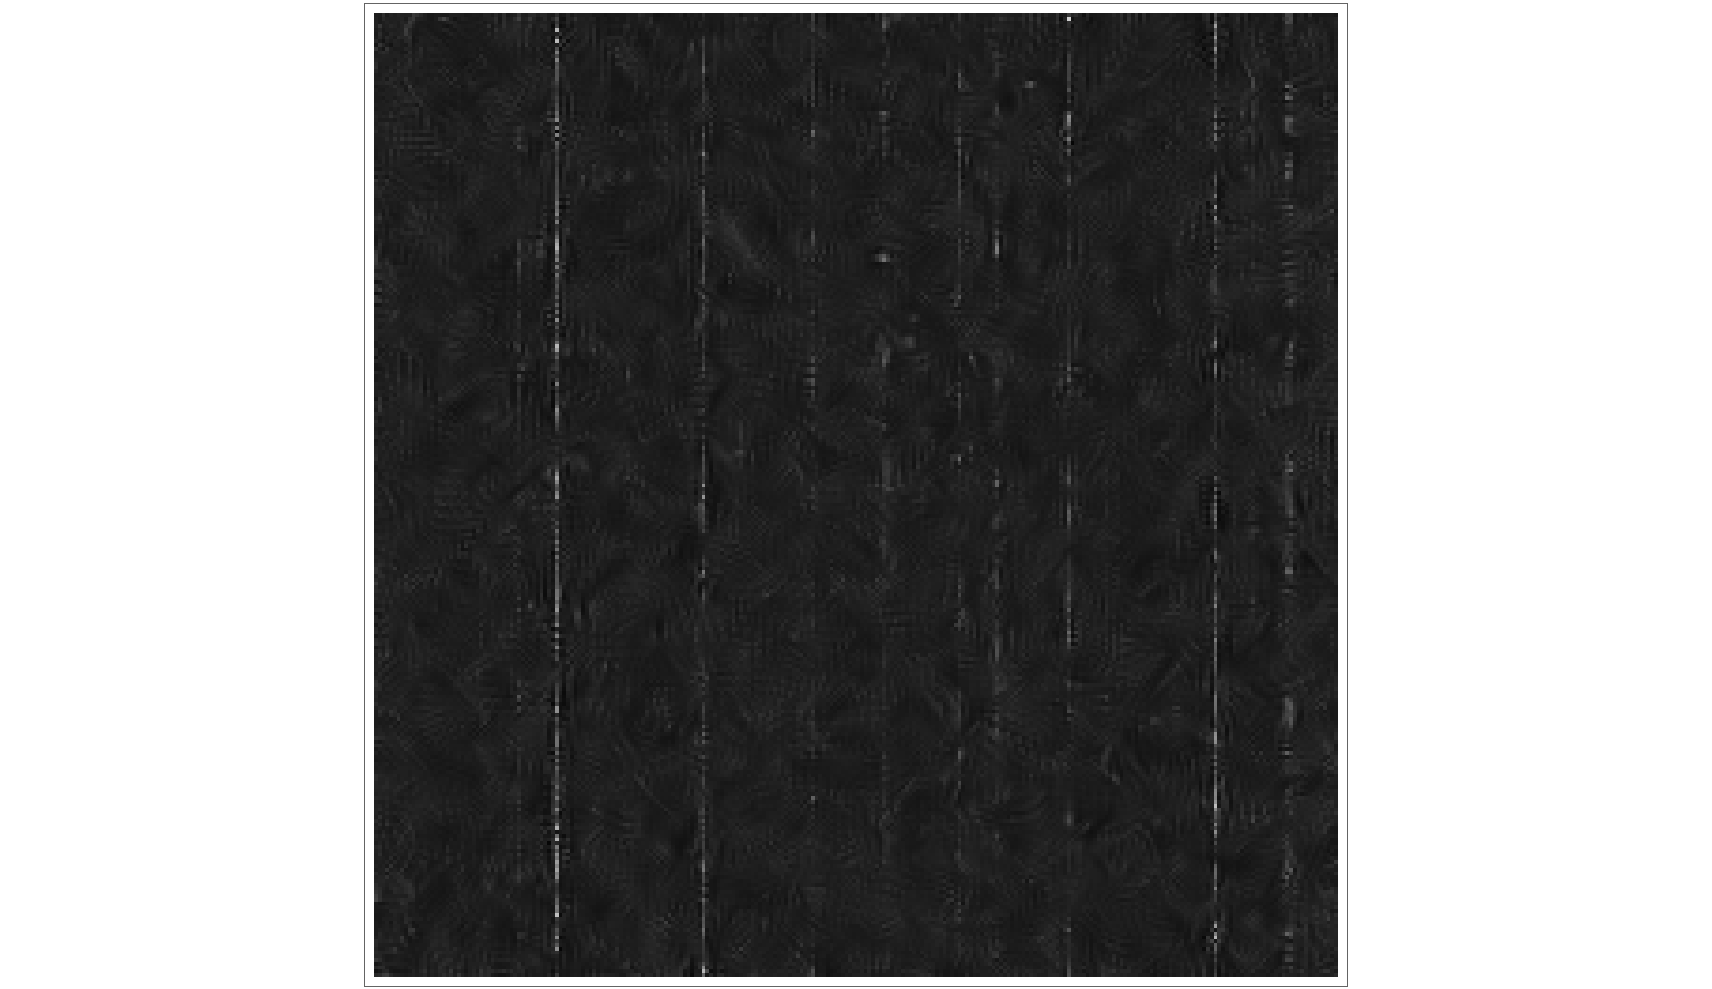
\includegraphics[width=0.8\linewidth]{../Data/pre-experiment/MRI_result_TR_0500_TE320.bmp}
    \caption{$T_R = \text{\si{500 \micro\second}}, T_E = \text{\si{320 \micro\second}}$时的自旋回波序列共振成像结果}
    \label{fig:mri_0500_320}
\end{figure}

\begin{figure}[H]
    \centering
    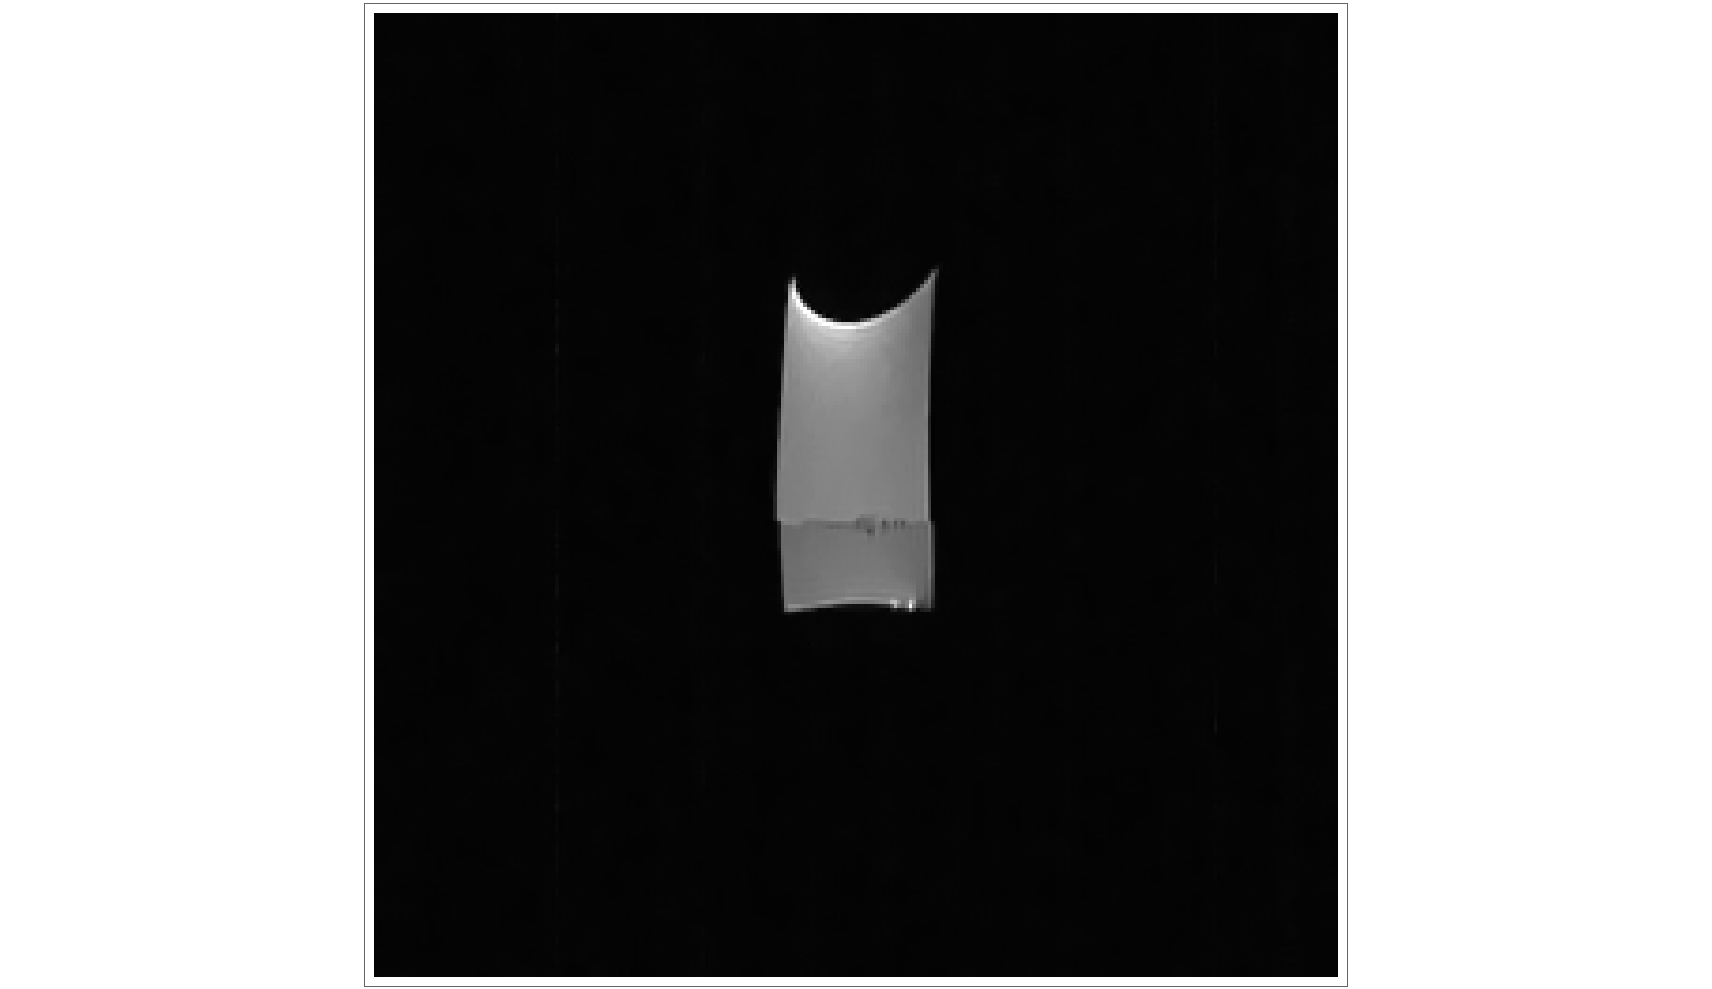
\includegraphics[width=0.8\linewidth]{../Data/pre-experiment/MRI_result_TR_1000_TE_020.bmp}
    \caption{$T_R = \text{\si{1000 \micro\second}}, T_E = \text{\si{20 \micro\second}}$时的自旋回波序列共振成像结果}
    \label{fig:mri_1000_020}
\end{figure}

从图\ref{fig:mri_0500_020}、\ref{fig:mri_0500_040}、\ref{fig:mri_0500_160}再到图\ref{fig:mri_0500_320}的对照中可以看出,随着$T_E$不断提高,$T_2$差别对成像相对信号的影响逐渐显现出来,上部的食用油因其横向弛豫时间$T_2$较长而在成像中表现为高信号区域,而下部的硫酸铜溶液因其横向弛豫时间$T_2$较短而在成像中表现为低信号区域。同时,成像信噪比不断降低,这是因为随着$T_E$的增大,核自旋磁化矢量在$x-y$平面内发生横向弛豫的时间间隔也随之增大,导致回波信号的幅值逐渐减小。

从图\ref{fig:mri_0060_020}、\ref{fig:mri_0260_020}、\ref{fig:mri_0500_020}的对照中可以看出,随着$T_R$不断减小,纵向弛豫时间$T_1$差别对成像相对信号的影响逐渐变得显著,下部的硫酸铜溶液因其纵向弛豫时间$T_1$较短而在成像中表现为高信号区域,而上部的食用油因其纵向弛豫时间$T_1$较长而在成像中表现为低信号区域。同时,成像信噪比也逐渐降低,这是因为随着$T_R$的减小,核自旋磁化矢量在$z$轴方向难以完全恢复到平衡状态,导致回波信号的幅值逐渐减小。

综合以上分析,可以确认,图\ref{fig:mri_0500_020}近似实现了质子密度加权成像,图\ref{fig:mri_0060_020}近似实现了横向弛豫时间$T_2$加权成像,图\ref{fig:mri_0500_160}近似实现了纵向弛豫时间$T_1$加权成像。

% \section{结论}


%%%%%%%%%%%%%%%%%%%%%%%%%%%%%%%%%%%%%%%%%%%%%%%%%%%%%%%%%%%%%%%%
%  参考文献
%%%%%%%%%%%%%%%%%%%%%%%%%%%%%%%%%%%%%%%%%%%%%%%%%%%%%%%%%%%%%%%%
%  参考文献按GB/T 7714-2015《文后参考文献著录规则》的要求著录. 
%  参考文献在正文中的引用方法:\cite{bib文件条目的第一行}

\renewcommand\refname{\heiti\wuhao\centerline{参考文献}\global\def\refname{参考文献}}
\vskip 12pt


\let\OLDthebibliography\thebibliography
\renewcommand\thebibliography[1]{
  \OLDthebibliography{#1}
  \setlength{\parskip}{0pt}
  \setlength{\itemsep}{0pt plus 0.3ex}
}

{
\renewcommand{\baselinestretch}{0.9}
\liuhao
\bibliographystyle{gbt7714-numerical}
\bibliography{./Report/TempExample}
}

\appendix
\section{衍射谱寻峰数据}


\end{document}
